% !TEX root = ferguson-proposal.tex
\chapter{Overview}
\label{sec:overview}

We first present an overview of \sys, including the model of
interaction, the types of messages, and the kinds of network resources
one can request. We discuss the challenges involved in exposing
network control to multiple principals, and the solutions we
propose. We then discuss additional considerations that influenced
\sys's design, which we detail in the following chapters
(\ref{sec:messages}-\ref{sec:FullSystem}).

\vskip 1em

\sys allows principals to gain controlled visibility into the network
and to safely influence network operations.  \emph{Principals} in \sys
are end users, or, most commonly, applications and devices running on
their behalf. 
We assume some infrastructure in the network for authentication,
such as 802.1x associated with an existing user database.
After authentication, principals interact with the \sys
controller using a simple text-based protocol.

Principals can issue three types of messages to read and write network
state: \emph{requests} (\xref{sec:Requests}), \emph{queries}
(\xref{sec:Queries}), and \emph{hints} (\xref{sec:Hints}).  Requests
are for resources (\eg, bandwidth or access control), with an action
to be taken by the controller. Queries read some component of network
state (\eg, traffic between hosts, or available bandwidth). Hints
inform \sys about current or future traffic characteristics; the
controller may choose to use hints to improve service. Our initial
design implements a first come-first serve service model, where the
controller handles messages in a serialized fashion.

Each message refers to some subset of the network's flows; we call
these \emph{flowgroups}. For example, a message may request to deny
all traffic from a particular host, or to rate-limit a single
flow, or query the bandwidth used by some set of flows. Without
restrictions, a malicious or negligent principal can adversely affect
the network -- a key novelty of \sys is its method to safely allow multiple
principals to affect the network, without ceding administrative
privileges.

%% Keep for posterity:
As simple examples, a firewall program in a user's machine may issue a 
request for denying all traffic from external IP addresses to
itself, to be implemented at the edges of the network; a distributed
RPC library may issue a hint for the network informing that all
flows between two ports will be small flows; or a backup application
may query the network about the current buffer utilizations along a 
path. 

\sys's design addresses two key challenges. First, it provides a flexible
mechanism that gives multiple principals control
over a fine-grained portion of network resources. Second, it resolves
the inevitable conflicts that arise between principals' requests, while
allowing oversubscription.

\vskip 1em

\begin{figure}[t]
\centering
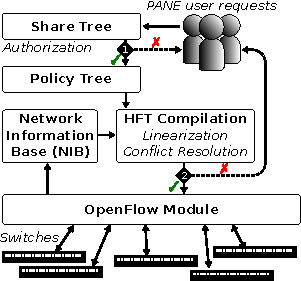
\includegraphics[width=0.3\textwidth]{figs/compilation-pane}
\caption{The \sys system and request processing}
\label{f:system}
\end{figure}

\tightparagraph{Limiting Authority}
\sys uses \emph{shares} to limit the authority of principals.  A share
states \emph{who} (which principals) can say \emph{what} (which
messages) about \emph{which} flows in the network.  This statement is
represented, respectively, by a share's three components: its
\emph{principals}, \emph{privileges}, and \emph{flowgroup}.
Figure~\ref{fig:shares}(a) shows an example share.  Principals of a
share have two implicit privileges. A principal can delegate its
privileges to another principal, much like passing an object
capability. In addition, principals can create sub-shares of shares to
which they have access. Shares are thus organized in a global
\emph{share tree}. The share tree enforces two key invariants: a
sub-share's flowgroup must be a subset of its parent's flowgroup, and a
sub-share's privileges cannot be more permissive than its parent
share's privileges.

Figure \ref{fig:interaction-example} traces an example interaction
in which the root user creates a new share, \verb/aliceBW/ restricted to Alice's traffic (Line 1).
This share carries the privilege to reserve up to 10 Mbps of guaranteed
minimum bandwidth, and is a sub-share of the root share. In Line 2,
the root user grants Alice access to this share. Alice then uses this
share to reserve bandwidth for her HTTP (port 80) flows for 10 minutes,
starting 20 minutes in the future (Line 3). In the next line, the root
user creates a share for traffic destined to Bob's computer (\verb/10.0.0.2/)
with the privilege to deny traffic, and subsequently grants Bob access
to this share (Line 5). In Line 6, Bob successfully uses this share to block
access from a host \verb/10.0.0.3/ for five minutes. However, his attempt to
block traffic from that host to \verb/10.0.0.4/ is rejected as the specified
flow group is not a subset of the share's flowgroup (\verb/dstHost=10.0.0.2/).

\vskip 1em

%[Maybe here comes a short version of the interaction example?]
\begin{figure}[t]
\begin{boxedminipage}{\columnwidth}
\begin{small}
\begin{Verbatim}
1 root: NewShare aliceBW for (user=Alice) [reserve <= 10Mb] on rootShare.
2 root: Grant aliceBW to Alice.
3 Alice: reserve(user=Alice,dstPort=80) = 8Mb on aliceBW from +20min to +30min.
4 root: NewShare bobAC for (dstHost=10.0.0.2) [deny = True] on rootShare.
5 root: Grant bobAC to Bob.
6 Bob: deny(dstHost=10.0.0.2, srcHost=10.0.0.3) on bobAC from now to +5min.
7 Bob: deny(dstHost=10.0.0.4, srcHost=10.0.0.3) on bobAC.
\end{Verbatim}
\end{small}
\end{boxedminipage}
\caption{Sample interaction between three principals and \sys.}
\label{fig:interaction-example}
\end{figure}

\tightparagraph{Resolving Conflicts}
The share tree constrains the policies that can be realized in the
network, but does not itself cause any policy to be implemented in the
network. Instead, accepted requests and realized hints determine
network policy.  We call such accepted requests and realized hints
\emph{policy atoms} -- units of the overall network policy.  Policy
atoms are arranged in the same hierarchy as the share tree, forming a
\emph{policy tree}.  A policy tree is a declarative data structure
that represents the desired global policy for the network. \sys
materializes this policy in the network by installing rules in the
switches that implement an equivalent policy (\xref{sec:FullSystem}).

Policy atoms thus exist in the context of a share, and are bound by the
shares' privileges and flowgroup. However, policy atoms may
conflict.  For example, one policy atom may deny all HTTP flows, while
another allows HTTP flows. These atoms may even exist on
different shares. The \sys share tree is flexible: it supports
oversubscription, and allows several shares to express policies for
overlapping flowgroups.  A key novelty of \sys is a principled and
intuitive \emph{conflict-resolution} algorithm for hierarchical
policies.

We develop Hierarchical Flow Tables (HFTs) to materialize \sys's policy tree.  HFTs
provide a model for resolving conflicts in a hierarchy of policies,
and a formally-verified compiler from such hierarchies to flow tables
suitable for OpenFlow switches.  In particular, HFTs use
\emph{conflict resolution operators} within and between each node in
the hierarchy to flexibly resolve conflicts. We describe the design
of \sys's operators, and the semantics and implementation of HFTs in
\xref{sec:conflicts}.

\vskip 1em

\tightparagraph{Request Processing}
Having summarized \sys's key ideas, we now describe at a high level the
processing of a single request, as depicted in
Figure~\ref{f:system}. When an authenticated principal sends the controller a
message, perhaps requesting a resource for a flowgroup in a particular
share, \sys first checks that the request is admissible per the share's
flowgroup and privileges -- Check 1 in the figure.

If this first check passes, \sys then checks to see if it is
compatible with the state of the network -- Check 2. This check
involves all accepted requests (\ie, policy atoms) in the
policy tree, and the physical capabilities of the network. For
example, a bandwidth reservation requires a circuit between
two endpoints with sufficient bandwidth and switch queues.
This check requires compiling the current policy
tree, augmented with the request itself.  If this check passes, the
request is incorporated into the tree, and the controller can install
the policy onto the network.
This process also has a variation which only partially fulfills requests;
\xref{sec:strict-partial} describes both variations in more detail.

A final key feature, which we detail in subsequent chapters,
is that \sys allows principals to request resources for future intervals.
To support this, \sys maintains a time-indexed sequence of policy trees. The above
checks may thus be made against future, planned network state as appropriate.



